\section{Introduction to Cryptdb}

This section introduces the structure of Cryptdb to show how data is duplicated. This introduction is based on the original paper and the newest verion of Cryptdb implementation. We would like to introduce the following content.

1. structure of client, proxy, and MySQL server\\

2. structure of metadata storage\\

3. datalayout \\

This section will give you insight on how we find duplicates in Cryptdb, and important issues to consider when designing a backup system.



\subsection{The client,server, proxy structure}

In the cryptdb system design, there are three identities, client, server, and proxy. The Client is the webserver, and the server has MySQL installed. The client communicate with the proxy instead of with the server. The MySQL server is not trusted while the Proxy is trusted. When the client receive DDL queries, it will stored related metadata to describe the encryption schema of each table. For both DML and DDL queries, the proxy perform query rewrite to encrypt the query and send encrypted query to MySQL server. The results are sent to the proxy first for decryption, and then plain text will be sent to client. Figure~\ref{fig:stack1} shows the basic structure of Cryptdb and the traditional database. 


\begin{figure}[tb]
\centering
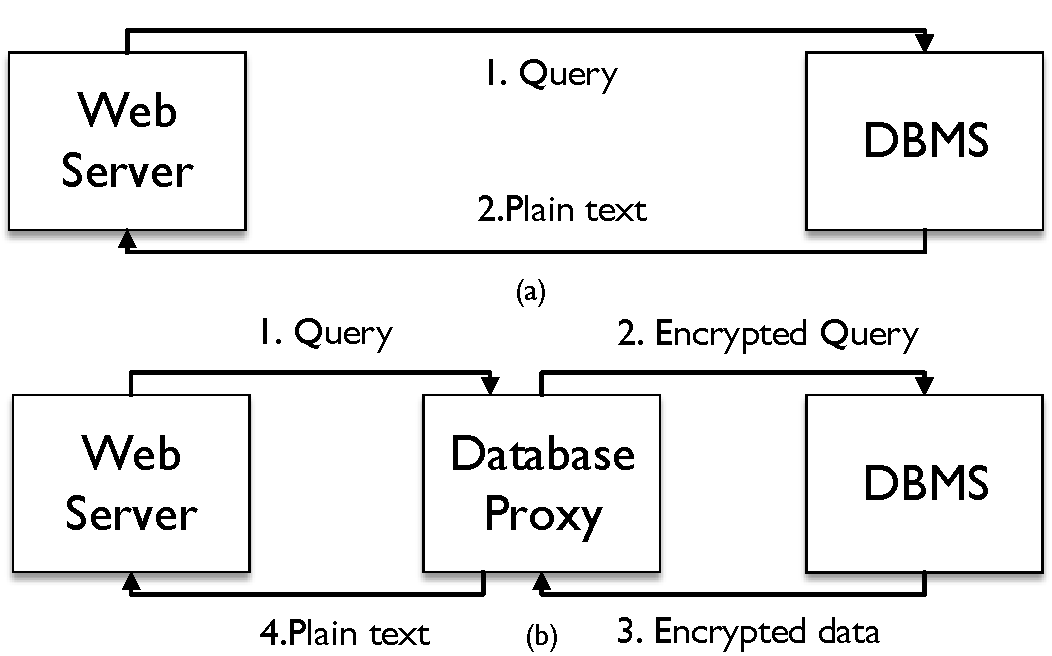
\includegraphics[width=6cm]{images/Cryptdb-structure.pdf}
\caption{structure of cryptdb}
\label{fig:stack1}
\end{figure}



\subsection{metadata layout and structure}

This section talks about metadata layout and the conresponding encryption scheme. Those scheme will impact how we make choices when we bakcup data. The metadata form a hirechy from the database level to the encryption layer level. It has a structure of a tree. Figure~\ref{fig:stack2} shows the structure of onionmeta.


\begin{figure}[tb]
\centering
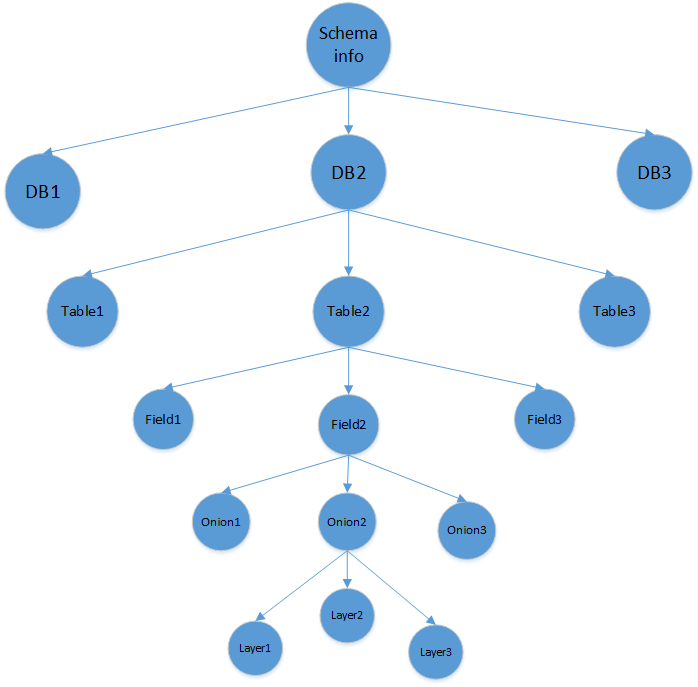
\includegraphics[width=4cm]{images/layers.png}
\caption{Onionmeta layout}
\label{fig:stack2}
\end{figure}

Every node in the tree is storaed as a record with a unique id in a relational table. The relation among nodes and the content of a node is also stored in the same table. Each onion represents an encryption scheme, which has many layers. This tree structure can be stored in a simple relational table, 

CREATE TABLE MetaObject(id bigint(20) unsigned auto\_increment, parent\_id bigint(20),serial\_key varbinary(500),serial\_object varbinary(500));  


So the metadata of databases, tables, fields, onions, layers are all serialized and stored in the proxy. Since the amount of data is related only to the number tables and the number of fields in those tables, the storage size is small. Also, metadata is needed for decryption and data recovery, so we use physical backup and do not deduplicate the metadata. Metadata is in the form is plaintext, so traditional deduplication techinques can work properly.

